%% uncomment to list all files in log
%\listfiles

\documentclass[12pt]{report}


\usepackage{fontspec}

%\setmainfont[Scale=MatchLowercase]{Lucida Bright}
%\setmonofont{FreeMono}
%\setmonofont{Source Code Pro}
\setmonofont[Scale=MatchLowercase]{Ubuntu Mono}

\usepackage[headings]{fullpage}

% national use characters 
%\usepackage{inputenc}

% ams mathematical symbols
\usepackage{amsmath,amssymb}

% added to support pandoc highlighting
\usepackage{microtype}

\usepackage{makeidx}

% add index and bibliographies to table of contents
\usepackage[nottoc]{tocbibind}

% postscript courier and times in place of cm fonts
%\usepackage{courier}
%\usepackage{times}

% extended coloring
\usepackage{color}
\usepackage[table,dvipsnames]{xcolor}
\usepackage{colortbl}

% advanced date formating
\usepackage{datetime}

%support pandoc code highlighting
\usepackage{fancyvrb}
\DefineShortVerb[commandchars=\\\{\}]{\|}
\DefineVerbatimEnvironment{Highlighting}{Verbatim}{commandchars=\\\{\}}
% Add ',fontsize=\small' for more characters per line

%tango style colors
% \usepackage{framed}
% \definecolor{shadecolor}{RGB}{255,255,255}
% \newenvironment{Shaded}{\begin{snugshade}}{\end{snugshade}}
% \newcommand{\KeywordTok}[1]{\textcolor[rgb]{0.13,0.29,0.53}{\textbf{{#1}}}}
% \newcommand{\DataTypeTok}[1]{\textcolor[rgb]{0.13,0.29,0.53}{{#1}}}
% \newcommand{\DecValTok}[1]{\textcolor[rgb]{0.00,0.00,0.81}{{#1}}}
% \newcommand{\BaseNTok}[1]{\textcolor[rgb]{0.00,0.00,0.81}{{#1}}}
% \newcommand{\FloatTok}[1]{\textcolor[rgb]{0.00,0.00,0.81}{{#1}}}
% \newcommand{\CharTok}[1]{\textcolor[rgb]{0.31,0.60,0.02}{{#1}}}
% \newcommand{\StringTok}[1]{\textcolor[rgb]{0.31,0.60,0.02}{{#1}}}
% \newcommand{\CommentTok}[1]{\textcolor[rgb]{0.56,0.35,0.01}{\textit{{#1}}}}
% \newcommand{\OtherTok}[1]{\textcolor[rgb]{0.56,0.35,0.01}{{#1}}}
% \newcommand{\AlertTok}[1]{\textcolor[rgb]{0.94,0.16,0.16}{{#1}}}
% \newcommand{\FunctionTok}[1]{\textcolor[rgb]{0.00,0.00,0.00}{{#1}}}
% \newcommand{\RegionMarkerTok}[1]{{#1}}
% \newcommand{\ErrorTok}[1]{\textbf{{#1}}}
% \newcommand{\NormalTok}[1]{{#1}}

%espresso style colors
% \usepackage{framed}
% \definecolor{shadecolor}{RGB}{42,33,28}
% \newenvironment{Shaded}{\begin{snugshade}}{\end{snugshade}}
% \newcommand{\KeywordTok}[1]{\textcolor[rgb]{0.26,0.66,0.93}{\textbf{{#1}}}}
% \newcommand{\DataTypeTok}[1]{\textcolor[rgb]{0.74,0.68,0.62}{\underline{{#1}}}}
% \newcommand{\DecValTok}[1]{\textcolor[rgb]{0.27,0.67,0.26}{{#1}}}
% \newcommand{\BaseNTok}[1]{\textcolor[rgb]{0.27,0.67,0.26}{{#1}}}
% \newcommand{\FloatTok}[1]{\textcolor[rgb]{0.27,0.67,0.26}{{#1}}}
% \newcommand{\CharTok}[1]{\textcolor[rgb]{0.02,0.61,0.04}{{#1}}}
% \newcommand{\StringTok}[1]{\textcolor[rgb]{0.02,0.61,0.04}{{#1}}}
% \newcommand{\CommentTok}[1]{\textcolor[rgb]{0.00,0.40,1.00}{\textit{{#1}}}}
% \newcommand{\OtherTok}[1]{\textcolor[rgb]{0.74,0.68,0.62}{{#1}}}
% \newcommand{\AlertTok}[1]{\textcolor[rgb]{1.00,1.00,0.00}{{#1}}}
% \newcommand{\FunctionTok}[1]{\textcolor[rgb]{1.00,0.58,0.35}{\textbf{{#1}}}}
% \newcommand{\RegionMarkerTok}[1]{\textcolor[rgb]{0.74,0.68,0.62}{{#1}}}
% \newcommand{\ErrorTok}[1]{\textcolor[rgb]{0.74,0.68,0.62}{\textbf{{#1}}}}
% \newcommand{\NormalTok}[1]{\textcolor[rgb]{0.74,0.68,0.62}{{#1}}}

%kete style colors
% \newenvironment{Shaded}{}{}
% \newcommand{\KeywordTok}[1]{\textbf{{#1}}}
% \newcommand{\DataTypeTok}[1]{\textcolor[rgb]{0.50,0.00,0.00}{{#1}}}
% \newcommand{\DecValTok}[1]{\textcolor[rgb]{0.00,0.00,1.00}{{#1}}}
% \newcommand{\BaseNTok}[1]{\textcolor[rgb]{0.00,0.00,1.00}{{#1}}}
% \newcommand{\FloatTok}[1]{\textcolor[rgb]{0.50,0.00,0.50}{{#1}}}
% \newcommand{\CharTok}[1]{\textcolor[rgb]{1.00,0.00,1.00}{{#1}}}
% \newcommand{\StringTok}[1]{\textcolor[rgb]{0.87,0.00,0.00}{{#1}}}
% \newcommand{\CommentTok}[1]{\textcolor[rgb]{0.50,0.50,0.50}{\textit{{#1}}}}
% \newcommand{\OtherTok}[1]{{#1}}
% \newcommand{\AlertTok}[1]{\textcolor[rgb]{0.00,1.00,0.00}{\textbf{{#1}}}}
% \newcommand{\FunctionTok}[1]{\textcolor[rgb]{0.00,0.00,0.50}{{#1}}}
% \newcommand{\RegionMarkerTok}[1]{{#1}}
% \newcommand{\ErrorTok}[1]{\textcolor[rgb]{1.00,0.00,0.00}{\textbf{{#1}}}}
% \newcommand{\NormalTok}[1]{{#1}}
%end pandoc code hacks

% jodliterate colors
\usepackage{color}
\definecolor{shadecolor}{RGB}{248,248,248}
% j control structures 
\definecolor{keywcolor}{rgb}{0.13,0.29,0.53}
% j explicit arguments x y m n u v
\definecolor{datacolor}{rgb}{0.13,0.29,0.53}
% j numbers - all types see j.xml
\definecolor{decvcolor}{rgb}{0.00,0.00,0.81}
\definecolor{basencolor}{rgb}{0.00,0.00,0.81}
\definecolor{floatcolor}{rgb}{0.00,0.00,0.81}
% j local assignments
\definecolor{charcolor}{rgb}{0.31,0.60,0.02}
\definecolor{stringcolor}{rgb}{0.31,0.60,0.02}
\definecolor{commentcolor}{rgb}{0.56,0.35,0.01}
% primitive adverbs and conjunctions
%\definecolor{othercolor}{rgb}{0.56,0.35,0.01}   
\definecolor{othercolor}{RGB}{0,0,255}
% global assignments
\definecolor{alertcolor}{rgb}{0.94,0.16,0.16}
% primitive J verbs and noun names
\definecolor{funccolor}{rgb}{0.00,0.00,0.00}    

\usepackage{framed}
\newenvironment{Shaded}{}{}
\newcommand{\KeywordTok}[1]{\textcolor{keywcolor}{\textbf{{#1}}}}
\newcommand{\DataTypeTok}[1]{\textcolor{datacolor}{{#1}}}
%\newcommand{\DecValTok}[1]{\textcolor{decvcolor}{{#1}}}
\newcommand{\DecValTok}[1]{{#1}} 
\newcommand{\BaseNTok}[1]{\textcolor{basencolor}{{#1}}}
\newcommand{\FloatTok}[1]{\textcolor{floatcolor}{{#1}}}
\newcommand{\CharTok}[1]{\textcolor{charcolor}{\textbf{{#1}}}}
\newcommand{\StringTok}[1]{\textcolor{stringcolor}{{#1}}}
\newcommand{\CommentTok}[1]{\textcolor{commentcolor}{\textit{{#1}}}}
\newcommand{\OtherTok}[1]{\textcolor{othercolor}{{#1}}} 
\newcommand{\AlertTok}[1]{\textcolor{alertcolor}{\textbf{{#1}}}}
%\newcommand{\FunctionTok}[1]{\textcolor{funccolor}{{#1}}}
\newcommand{\FunctionTok}[1]{{#1}}
\newcommand{\RegionMarkerTok}[1]{{#1}}
\newcommand{\ErrorTok}[1]{\textbf{{#1}}}
\newcommand{\NormalTok}[1]{{#1}}

% headers and footers
\usepackage{fancyhdr}
\pagestyle{fancy}

\fancyhead{}
\fancyfoot{}

%\fancyhead[LE,RO]{\slshape \rightmark}
%\fancyhead[LO,RE]{\slshape \leftmark}
\fancyfoot[C]{\thepage}
%\headrulewidth 0.4pt
%\footrulewidth 0 pt

%\addtolength{\headheight}{\baselineskip}

%\lfoot{\emph{Analyze the Data not the Drivel}}
%\rfoot{\emph{\today}}

% subfigure handles figures that contain subfigures
%\usepackage{color,graphicx,subfigure,sidecap}
\usepackage{graphicx,sidecap}
\usepackage{subfigure}
\graphicspath{{./inclusions/}}

% floatflt provides for text wrapping around small figures and tables
\usepackage{floatflt}

% tweak caption formats 
\usepackage{caption} 
\usepackage{sidecap}
%\usepackage{subcaption} % not compatible with subfigure

\usepackage{rotating} % flip tables sideways

% complex footnotes
%\usepackage{bigfoot}

% weird logos \XeLaTeX
\usepackage{metalogo}

% source code listings
\usepackage{listings}

% long tables
% \usepackage{longtable}

\newcommand{\HRule}{\rule{\linewidth}{0.5mm}}

% map LaTeX cross references into PDF cross references
\usepackage[
            %dvips,
            colorlinks,
            linkcolor=blue,
            citecolor=blue,
            urlcolor=blue,   % magenta, cyan default        
            pdfauthor={John D. Baker},
            pdftitle={Analyze the Data not the Drivel},
            pdfsubject={Blog},
            pdfcreator={MikTeX+LaTeXe with hyperref package},
            pdfkeywords={blog,wordpress},
            ]{hyperref}
           
% custom colors
\definecolor{CodeBackGround}{cmyk}{0.0,0.0,0,0.05}    % light gray
\definecolor{CodeComment}{rgb}{0,0.50,0.00}           % dark green {0,0.45,0.08}
\definecolor{TableStripes}{gray}{0.9}                 % odd/even background in tables

\lstdefinelanguage{bat}
{morekeywords={echo,title,pushd,popd,setlocal,endlocal,off,if,not,exist,set,goto,pause},
sensitive=True,
morecomment=[l]{rem}
}

\lstdefinelanguage{jdoc}
{
morekeywords={},
otherkeywords={assert.,break.,continue.,for.,do.,if.,else.,elseif.,return.,select.,end.
,while.,whilst.,throw.,catch.,catchd.,catcht.,try.,case.,fcase.},
sensitive=True,
morecomment=[l]{NB.},
morestring=[b]',
morestring=[d]',
}

% latex size ordering - can never remember it
% \tiny
% \scriptsize
% \footnotesize
% \small
% \normalsize
% \large
% \Large
% \LARGE
% \huge
% \Huge
 
% listings package settings  
\lstset{%
  language=jdoc,                                % j document settings
  basicstyle=\ttfamily\footnotesize,            
  keywordstyle=\bfseries\color{keywcolor}\footnotesize,
  identifierstyle=\color{black},
  commentstyle=\slshape\color{CodeComment},     % colored slanted comments
  stringstyle=\color{red}\ttfamily,
  showstringspaces=false,                       
  %backgroundcolor=\color{CodeBackGround},       
  frame=single,                                
  framesep=1pt,                                 
  framerule=0.8pt,                             
  rulecolor=\color{CodeBackGround},   
  showspaces=false,
  %columns=fullflexible,
  %numbers=left,
  %numberstyle=\footnotesize,
  %numbersep=9pt,
  tabsize=2,
  showtabs=false,
  captionpos=b
  breaklines=true,                              
  breakindent=5pt                              
}

\lstdefinelanguage{JavaScript}{
  keywords={typeof, new, true, false, catch, function, return, null, catch, switch, var, if, in, while, do, else, case, break},
  ndkeywords={class, export, boolean, throw, implements, import, this},
  ndkeywordstyle=\color{darkgray}\bfseries,
  sensitive=false,
  comment=[l]{//},
  morecomment=[s]{/*}{*/},
  morestring=[b]',
  morestring=[b]"
}

% C# settings
\lstdefinestyle{sharpc}{
language=[Sharp]C,
basicstyle=\ttfamily\scriptsize, 
keywordstyle=\bfseries\color{keywcolor}\scriptsize,
framerule=0pt
}

% for source code listing longer than two use smaller font
\lstdefinestyle{smallersource}{
basicstyle=\ttfamily\scriptsize, 
keywordstyle=\bfseries\color{keywcolor}\scriptsize,
framerule=0pt
}

\lstdefinestyle{resetdefaults}{
language=jdoc,
basicstyle=\ttfamily\footnotesize,  
keywordstyle=\bfseries\color{keywcolor}\footnotesize,                                                               
framerule=0.8pt 
}

% APL UTF8 code points listed for lstlisting processing
\makeatletter
\lst@InputCatcodes
\def\lst@DefEC{%
 \lst@CCECUse \lst@ProcessLetter
  ^^80^^81^^82^^83^^84^^85^^86^^87^^88^^89^^8a^^8b^^8c^^8d^^8e^^8f%
  ^^90^^91^^92^^93^^94^^95^^96^^97^^98^^99^^9a^^9b^^9c^^9d^^9e^^9f%
  ^^a0^^a1^^a2^^a3^^a4^^a5^^a6^^a7^^a8^^a9^^aa^^ab^^ac^^ad^^ae^^af%
  ^^b0^^b1^^b2^^b3^^b4^^b5^^b6^^b7^^b8^^b9^^ba^^bb^^bc^^bd^^be^^bf%
  ^^c0^^c1^^c2^^c3^^c4^^c5^^c6^^c7^^c8^^c9^^ca^^cb^^cc^^cd^^ce^^cf%
  ^^d0^^d1^^d2^^d3^^d4^^d5^^d6^^d7^^d8^^d9^^da^^db^^dc^^dd^^de^^df%
  ^^e0^^e1^^e2^^e3^^e4^^e5^^e6^^e7^^e8^^e9^^ea^^eb^^ec^^ed^^ee^^ef%
  ^^f0^^f1^^f2^^f3^^f4^^f5^^f6^^f7^^f8^^f9^^fa^^fb^^fc^^fd^^fe^^ff%
  ^^^^20ac^^^^0153^^^^0152%
  ^^^^20a7^^^^2190^^^^2191^^^^2192^^^^2193^^^^2206^^^^2207^^^^220a%
  ^^^^2218^^^^2228^^^^2229^^^^222a^^^^2235^^^^223c^^^^2260^^^^2261%
  ^^^^2262^^^^2264^^^^2265^^^^2282^^^^2283^^^^2296^^^^22a2^^^^22a3%
  ^^^^22a4^^^^22a5^^^^22c4^^^^2308^^^^230a^^^^2336^^^^2337^^^^2339%
  ^^^^233b^^^^233d^^^^233f^^^^2340^^^^2342^^^^2347^^^^2348^^^^2349%
  ^^^^234b^^^^234e^^^^2350^^^^2352^^^^2355^^^^2357^^^^2359^^^^235d%
  ^^^^235e^^^^235f^^^^2361^^^^2362^^^^2363^^^^2364^^^^2365^^^^2368%
  ^^^^236a^^^^236b^^^^236c^^^^2371^^^^2372^^^^2373^^^^2374^^^^2375%
  ^^^^2377^^^^2378^^^^237a^^^^2395^^^^25af^^^^25ca^^^^25cb%  
  ^^00}
\lst@RestoreCatcodes
\makeatother

% custom lengths used within minipages
\newcommand{\minindent}{17pt}


\makeindex

\begin{document}

\subsection*{\href{http://bakerjd99.wordpress.com/2011/01/14/the-un-space-treaty-is-holding-us-back/}{The UN Space Treaty is Holding Us Back!}}
\addcontentsline{toc}{subsection}{The UN Space Treaty is Holding Us Back!}


\noindent\emph{Posted: 14 Jan 2011 21:55:24}
\vspace{6pt}


%{[}caption id=``'' align=``alignleft'' width=``207'' caption=``Apollo  Earthrise''{]}
%\href{http://bakerjd99.files.wordpress.com/2011/01/moonrise1.jpg}{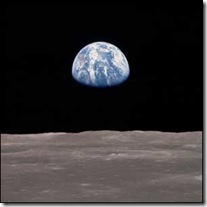
\includegraphics{moonrise_thumb1.jpg}}
%{[}/caption{]}
%\captionsetup[floatingfigure]{labelformat=empty}
%\begin{floatingfigure}[l]{0.25\textwidth}
%\centering
%\href{http://bakerjd99.files.wordpress.com/2011/01/moonrise1.jpg}{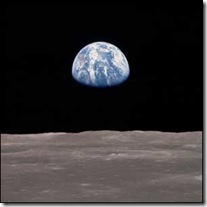
\includegraphics[width=0.23\textwidth]{moonrise_thumb1.jpg}}
%\caption{Apollo  Earthrise}
%\label{fig:1022X0}
%\end{floatingfigure} 


\captionsetup[figure]{labelformat=empty}
\begin{figure}[htbp]
\centering
\href{http://bakerjd99.files.wordpress.com/2011/01/moonrise1.jpg}{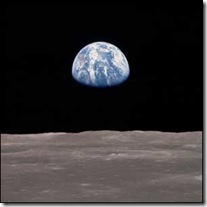
\includegraphics[width=0.23\textwidth]{moonrise_thumb1.jpg}}
\caption{Apollo  Earthrise}
\label{fig:1022X0}
\end{figure} 

2011 marks the \href{http://www.youtube.com/watch?v=aboZctrHfK8}{42}'nd
anniversary of the Apollo 11 moon landing. 42
\href{http://www.newser.com/story/comments/64908/moon-landing-denier-exposed-as-a-cheat.html}{idiot
infested} years have passed since that glorious day and nothing that has
happened since comes within a nautical league of matching it. My vile
boomer generation has downplayed the significance of space exploration
for decades. I remember getting a shrill lecture from my left leaning
fifth grade teacher about what a waste of money the space program was.
Being a self-assured child so I told my teacher he was preening
unimaginative Neanderthal. This landed me in detention but I refused to
apologize.

Manned space flight has been in a depressing, decades long, holding
pattern. The real advances in space exploration have come exclusively
from unmanned probes and robots. While astronauts have been going round
and round in that orbiting boondoggle known as the International Space
Station the \href{http://voyager.jpl.nasa.gov/}{Voyagers} are on the
brink of interstellar space, probes are on their way to
\href{http://pluto.jhuapl.edu/}{Pluto} and
\href{http://messenger.jhuapl.edu/}{Mercury},
\href{http://saturn.jpl.nasa.gov/}{Cassini} is orbiting Saturn, a small
armada of
\href{http://www.esa.int/SPECIALS/Mars\_Express/index.html}{orbiters}
and \href{http://marsrover.nasa.gov/home/}{crawlers} are exploring Mars,
low-budget missions discovered
\href{http://online.wsj.com/article/SB10001424052702303339504575566194097878552.html}{water
on the moon}, space telescopes like
\href{http://chandra.harvard.edu/}{Chandra},
\href{http://hubblesite.org/hubble\_20/}{Hubble} and
\href{http://www.spitzer.caltech.edu/}{Spitzer} have shown us wonder
after wonder and, capping it all off,
\href{http://map.gsfc.nasa.gov/}{WMAP} determined the age of the entire
frigging universe. Compare these awesome achievements to ISS astronauts
\href{http://www.nationalledger.com/cgi-bin/artman/exec/view.cgi?archive=26\&num=20926}{unplugging
zero-G toilets}.

Why has so little been accomplished? I can think of two good reasons.

\begin{enumerate}
\item
  Exclusive government control
\item
  The UN Space Treaty
\end{enumerate}
Until recently only governments could afford space programs. In the
early days of space exploration government control made sense but that
era is \href{http://www.spacex.com/}{coming to an end}. In a few decades
private entities will be able to mount manned Mars expeditions and send
robots anywhere in the solar system and beyond. The technology is coming
along nicely but I am afraid the politics will soon be a gigantic
millstone around our necks. The millstone takes the form of the
\href{http://www.oosa.unvienna.org/oosa/SpaceLaw/outerspt.html}{absurd
UN Space Treaty}.


%{[}caption id=``'' align=``alignright'' width=``244'' caption=``Green:  UN Space Treaty  nations''{]}
%\href{http://en.wikipedia.org/wiki/Outer\_Space\_Treaty}{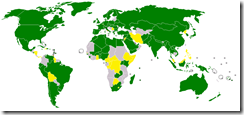
\includegraphics{800pxouter_space_treaty_thumb.png}}
%{[}/caption{]}
\captionsetup[figure]{labelformat=empty}
\begin{figure}[htbp]
\centering
\href{http://en.wikipedia.org/wiki/Outer\_Space\_Treaty}{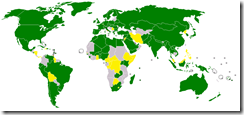
\includegraphics[width=0.45\textwidth]{800pxouter_space_treaty_thumb.png}}
\caption{Green:  UN Space Treaty  nations}
\label{fig:1022X1}
\end{figure} 

The UN space treaty is another sorry artifact of the 1960's. It reads
like a bunch of unwashed socialist hippies got together and decided to
ban capitalism in space. There is no other way to explain ridiculous
terms like:

\begin{enumerate}
\item
  \emph{The exploration and use of outer space shall be carried out for
  the benefit and in the interests of all countries and shall be the
  province of all mankind}.
\item
  \emph{Outer space is not subject to national appropriation by claim of
  sovereignty, by means of use or occupation, or by any other means.}
\item
  \emph{States shall be responsible for national space activities
  whether carried out by governmental or non-governmental activities.}
\item
  \emph{States shall be liable for damage caused by their space
  objects.}
\item
  \emph{States shall avoid harmful contamination of space and celestial
  bodies.}
\end{enumerate}
Suppose some daring entrepreneur decides to mount an asteroid mining
expedition. This is not as crazy as it sounds. Asteroids are relatively
easy to get to and very easy to get off of. They also contain
\href{http://news.bbc.co.uk/2/hi/sci/tech/401227.stm}{mountains of
valuable rare earths, platinum and gold.} Eros alone holds well over
\href{http://www.suite101.com/content/economic-impact-of-asteroids-space-exploration-a187015}{20
trillion dollars} of metals. You could pay off the US national debt by
mining one dinky asteroid! One day, not very long from now, robot
asteroid mining will make a compelling business case. To bad the UN
Space Treaty outlaws it.

If you have to pay off all of mankind (\#1, \#2) your compelling
business case evaporates. Environmentalists, (yeah space
environmentalists), would complain that mining damages and contaminates
a celestial body (\#4, \#5). Finally, even if the operation was 100\%
privately funded, various governments could legally ransom our daring
entrepreneur or shut him down (\#3). These tactics have already been
tried. Remember the
\href{http://articles.latimes.com/1997/oct/01/local/me-37979}{hysteria
that preceded the launch of Cassini}. A pack of morons decided that the
\href{http://en.wikipedia.org/wiki/Radioisotope\_thermoelectric\_generator}{Plutonium
powered RTG} on Cassini posed a grave threat to all mankind and started
citing \href{http://www.animatedsoftware.com/cassini/trea9704.htm}{the
UN Space Treaty in hopes of blocking the launch}. Cassini was not a
money-making operation so we ignored the loons. Asteroid mining will be
another thing all together. Everyone will want their cut. With the UN in
charge we're going to feel like the \emph{probed} subjects in this Kids
in Hall video.

%\href{http://www.youtube.com/watch?v=xz7sBTHtcLU}{NIMP: Get screen shot of this video}
\begin{figure}[htbp]
\centering
\href{http://www.youtube.com/watch?v=xz7sBTHtcLU}{
\includegraphics[width=0.25\textwidth]{analprobingaliens.jpg}}
\caption{Click for anal probing aliens}
\label{fig:analprobe}
\end{figure}





%{[}youtube=http://www.youtube.com/watch?v=xz7sBTHtcLU\&feature=player\_embedded\#!{]}


%\captionsetup[floatingfigure]{labelformat=empty}
%\begin{figure}[htbp]
%\begin{floatingfigure}[l]{0.25\textwidth}
%\centering
%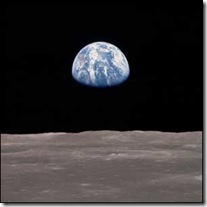
\includegraphics[width=0.23\textwidth]{moonrise_thumb1.jpg}
%\caption{~~~IMCAPTION~~~}
%\label{fig:1022X0}
%\end{floatingfigure}
%\end{figure}

%\captionsetup[floatingfigure]{labelformat=empty}
%\begin{figure}[htbp]
%\begin{floatingfigure}[l]{0.25\textwidth}
%\centering
%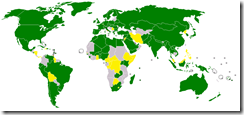
\includegraphics[width=0.23\textwidth]{800pxouter_space_treaty_thumb.png}
%\caption{~~~IMCAPTION~~~}
%\label{fig:1022X1}
%\end{floatingfigure}
%\end{figure}


%\end{document}